% (c) 2002 Matthew Boedicker <mboedick@mboedick.org> (original author) http://mboedick.org
% (c) 2003-2007 David J. Grant <davidgrant-at-gmail.com> http://www.davidgrant.ca
% (c) 2008 Nathaniel Johnston <nathaniel@nathanieljohnston.com> http://www.nathanieljohnston.com
% (l) 2012 Arun I B <arunib@smail.iitm.ac.in> http://www.ee.iitm.ac.in/~ee10s026/
%This work is licensed under the Creative Commons Attribution-Noncommercial-Share Alike 2.5 License. To view a copy of this license, visit http://creativecommons.org/licenses/by-nc-sa/2.5/ or send a letter to Creative Commons, 543 Howard Street, 5th Floor, San Francisco, California, 94105, USA.

\documentclass[letterpaper,11pt]{article}
\newlength{\outerbordwidth}
\pagestyle{empty}
\raggedbottom
\raggedright
\usepackage[svgnames]{xcolor}
\usepackage{framed}
\usepackage{times}
\usepackage{tocloft}
\usepackage{graphicx}
\usepackage{multirow}
\usepackage[utf8]{inputenc}
\usepackage{tabularx}
\usepackage[hidelinks]{hyperref}
\title{PAPER-CV}
%-----------------------------------------------------------
%Edit these values as you see fit

\setlength{\outerbordwidth}{3pt}  % Width of border outside of title bars
\definecolor{shadecolor}{gray}{0.75}  % Outer background color of title bars (0 = black, 1 = white)
\definecolor{shadecolorB}{gray}{0.93}  % Inner background color of title bars


%-----------------------------------------------------------
%Margin setup

\setlength{\evensidemargin}{-0.25in}
\setlength{\headheight}{-0.65in}
\setlength{\headsep}{0in}
\setlength{\oddsidemargin}{-0.25in}
\setlength{\paperheight}{11in}
\setlength{\paperwidth}{8.5in}
\setlength{\tabcolsep}{0in}
\setlength{\textheight}{11in}
\setlength{\textwidth}{7in}
\setlength{\topmargin}{-0.3in}
\setlength{\topskip}{0in}
\setlength{\voffset}{0in}


%-----------------------------------------------------------
%Custom commands
\newcommand{\comment}[1]{\ignorespaces}
\newcommand{\resitem}[1]{\item #1 \vspace{-2pt}}
\newcommand{\resheading}[1]{\vspace{0pt}
  \parbox{\textwidth}{\setlength{\FrameSep}{\outerbordwidth}
    \begin{shaded}
      \setlength{\fboxsep}{0pt}\framebox[\textwidth][l]{\setlength{\fboxsep}{4pt}\fcolorbox{shadecolorB}{shadecolorB}{\textbf{\sffamily{\mbox{~}\makebox[6.762in][l]{\large{\textsc{#1}}} \vphantom{p\^{E}}}}}}
    \end{shaded}
  }\vspace{-5pt}
}
\newcommand{\ressubheading}[4]{
  \begin{tabular*}{6.5in}{l@{\cftdotfill{\cftsecdotsep}\extracolsep{\fill}}r}
    \textbf{#1} & #2 \\
    \textit{#3} & \textit{#4} \\
  \end{tabular*}\vspace{-6pt}}
%-----------------------------------------------------------


\begin{document}

%-----------------------------------------------------------
\begin{tabular*}{7in}{l@{\extracolsep{\fill}}r}
  & \multirow{4}{*}{\rotatebox{270}{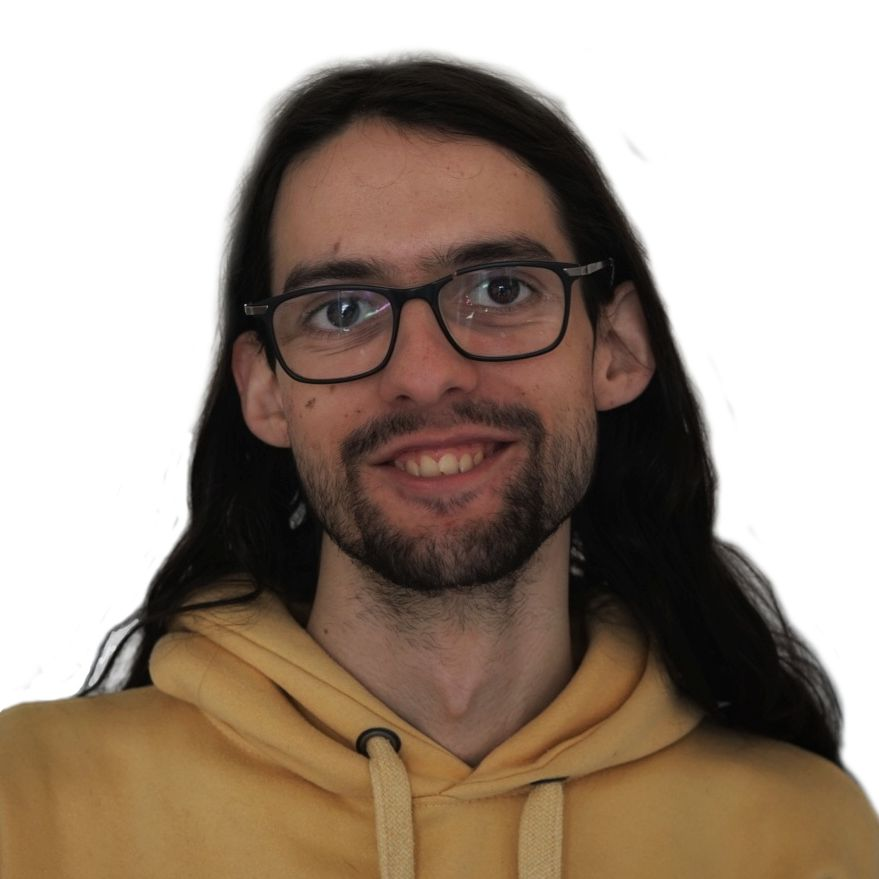
\includegraphics[width=3.4cm]{photo.JPG}}}\\
  & \\
  %-----------------------------------------------------------  
  \textbf{\Large Michael PAPER } & \\
  7 Quai Rouget de Lisle, 67000 Strasbourg, France  \\
  \href{mailto:michael.paper@ens-lyon.fr}{\texttt{michael.paper@ens-lyon.fr}} \\
  +33 6 69 56 80 99 \\
  Né le 27 Novembre 2000
\end{tabular*}
\\


%%%%%%%%%%%%%%%%%%%%%%%%%%%%%%
\resheading{Formation}
%%%%%%%%%%%%%%%%%%%%%%%%%%%%%%
\begin{itemize}
\item
  \ressubheading{ENS de Lyon}{Lyon, France}{Département
    d'Informatique}{Depuis septembre 2019}
  \begin{itemize}
    \resitem{Validation de la \textit{``Licence d'Informatique Fondamentale''}
      avec une moyenne de 16.502/20, 9ème place d'une promotion de 36
      étudiants}
    \resitem{Première année du \textit{``Master d'Informatique Fondamentale''}
      débuté en septembre 2020}
  \end{itemize}
  
\item
  \ressubheading{Université de Strasbourg}{Strasbourg, France}{UFR
    de Mathématique et d'Informatique}{2017 - 2019}
  \begin{itemize}
    \resitem{\textit{``Cursus de Master en Ingénierie : Informatique,
        Systèmes et Réseaux''} (CMI ISR)}
    \resitem{Validation de la L1 avec une moyenne de 14.692/20, 11ème
      place d'une promotion de plus de 200 étudiants}
    \resitem{Validation de la L2 avec une moyenne de 15.651/20, 2ème
      place d'une promotion de 74 étudiants}
  \end{itemize}
  
\item
  \ressubheading{Lycée Kléber}{Strasbourg, France}{Seconde à Terminale}{2014 - 2017}
  \begin{itemize}
    \resitem{Baccalauréat Scientifique, spécialité Mathématiques, mention Assez Bien (2017)}
  \end{itemize}
  
\end{itemize}


%%%%%%%%%%%%%%%%%%%%%%%%%%%%%%
\resheading{Expérience Professionnelle}
%%%%%%%%%%%%%%%%%%%%%%%%%%%%%%
\begin{itemize}
\item
  \ressubheading{INRIA Rennes
    (\texttt{\textmd{\href{https://www.inria.fr/}{https://www.inria.fr/}}})}{Rennes,
    France}{Stage de L3}{Juin-Juillet 2020}
  \begin{itemize}
    \resitem{Équipe Wide : \textit{Improving thread placement strategies for multicore processors with per-core frequency adaptation}}
  \end{itemize}

\item
  \ressubheading{Laboratoire ICube (\texttt{\textmd{\href{http://icube.unistra.fr/}{http://icube.unistra.fr/}}})}{Illkirch, France}{Stage optionnel de L2}{Juin 2019}
  \begin{itemize}
    \resitem{Section Spécifications, Contraintes et Preuves en Géométrie de l'équipe Informatique Géométrique et Graphique : preuves en Coq}
  \end{itemize}


 
\item
  \ressubheading{Talent Business Solutions (\texttt{\textmd{\href{https://www.talent-bs.com/}{https://www.talent-bs.com/}}})}{Strasboug, France}{Stage en entreprise de première année de CMI}{Juillet 2018}
  \begin{itemize}
    \resitem{Section Internet of Things : développement sur Microsoft Azure IoT Edge}
  \end{itemize}
  
  %\item 
  %	\ressubheading{Eurométropole de Strasbourg (\texttt{\textmd{\href{https://www.strasbourg.eu/}{https://www.strasbourg.eu/}}})}{Strasbourg, France}{Stage de collège}{Novembre 2013}
  %	\begin{itemize}
  %		\resitem{IT Department : création d'une page web animée entièrement en HTML5/CSS3}
  %	\end{itemize}
  
\end{itemize}



%%%%%%%%%%%%%%%%%%%%%%%%%%%%%%
\resheading{Compétences}
%%%%%%%%%%%%%%%%%%%%%%%%%%%%%%
\begin{itemize}
\item
  \textbf{Langages de programmation :} C, C++, OCaml, Haskell, MIPS, Coq, Javascript, Python, PHP
\item
  \textbf{Outils :} ArchLinux (i3wm/sway), GNU Make, Vim, Emacs, Git, LibreOffice, \LaTeX
\item
  \textbf{Projets :} voir \texttt{\textmd{\href{https://gitlab.com/HommeViande}{https://gitlab.com/HommeViande}}}
\item
  \textbf{Anglais :} courant, C1 advanced (CAE) validé en 2020
  
  
\end{itemize}


%%%%%%%%%%%%%%%%%%%%%%%%%%%%%%
\resheading{Activités diverses}
%%%%%%%%%%%%%%%%%%%%%%%%%%%%%%
\begin{itemize}
\item
  Speedcuber : Record personnel de 9.94s pour le Rubik's Cube $3\times3\times3$, résolution à l'aveugle, participation aux Championnats de France et aux Championnats du Monde de 2017 (\texttt{\href{https://www.worldcubeassociation.org/persons/2017PAPE04}{https://www.worldcubeassociation.org/persons/2017PAPE04}})
\item
  Cinéphile : Amateur de cinéma américain, français et coréen
  
\end{itemize}



\end{document}
